%%%%%%%%%%%%%%%%%%%%%%%%%%%%%%%%%%%%%%%%%%%%%%%%%%%%%%%%%%%%%

\mainmatter
\setcounter{page}{1}

\lectureseries[\course]{\course}

\auth[\lecAuth]{Lecturer: \lecAuth\\ Scribe: \scribe}
\date{September 24, 2009}

\setaddress

% the following hack starts the lecture numbering at 1
\setcounter{lecture}{0}
\setcounter{chapter}{0}

\lecture{Probability Review I}

\section{Types of Optimal Control}
Optimal control is concerned with reaching some specified goal that is given in advance. There is some flexibility in selecting the goal related to proposing a goal that is solvable and that can be considered correct for the operating regime, i.e., the goal must align with the desired outcome for the system. Optimal control is concerned with several types of dynamic systems:

\begin{itemize}
  \item Continuous and discrete time deterministic
  \item Continuous and discrete time stochastic
  \item Games
\end{itemize}

\subsection{Dynamics Representations}
Continuous time deterministic dynamics are given by
$$\dot\xi_t = f(\xi_t,u_t) \textnormal{, where } \xi_0 = x \in \mathbb{R}^n.$$
The state is represented as $\xi(t)$ and the control input is represented by $u(t)$.

Discrete time deterministic dynamics are generally known as ``classical optimal control'' dynamics and are given by
$$\xi_{t+1} = f(\xi_t,u_t).$$

Continuous time stochastic dynamics are given by
$$d\xi_t = f(\xi_t,u_t)dt + \sigma(\xi_t)dB_t.$$
Brownian motion is represented by $B$.

Discrete time stocahstic dynamics in continuous space are given by
$$\xi_{t+1} = f(\xi_t,u_t) + \sigma(\xi_t)w_t.$$
Random noise is represented by $w$.

Discrete time stocahstic dynamics in discrete space are given by
$$\xi_t \in \mathbb{X}.$$
The finite space is represented by $\mathbb{X}$ and this can be thought of as $\mathbb{N}$ or the set of all natural numbers.

The dynamics of games are given by
$$\dot\xi_t = f(\xi_t,u_t,w_t).$$
Player 1 is represented by $u$ and player 2 is represented by $w$.

\section{Applications}
\begin{table}[ht!]
\caption{Optimal Control Application Areas.}
\small
\centering
\begin{tabular}{@{}lllr@{}} \toprule
Discrete Time              & Continuous Time \\ \midrule
Machine repair/replacement & Vehicles        \\
Sensor Allocation          & Chemical plants \\
Job shops                  &                 \\
Command and control        &                 \\ \bottomrule
\end{tabular}
\label{tab:applications}
\end{table}

\section{Probability Review}
A set $\Omega$ is considered a sample space. We will be using $\sigma$-algebra in this course where $\Sigma$ is a $\sigma$-algebra of subsets of $\Omega$  and is defined by
\begin{align*}
&A \in \Sigma \textnormal{, } A^C \in \Sigma \\
&A,B \in \Sigma \Rightarrow A \cup B \in \Sigma \\
&A_i \in \Sigma ~\forall i \in \mathbb{N} \Rightarrow \bigcup_{i=1}^\infty A_i \in \Sigma.
\end{align*}
The term $A^C$ means the complement of $A$.

\begin{example}
\label{ex:cointoss}
Taking a fair coin and tossing it twice in a row has four possible outcomes that can be considered a set or a sample space such that
$$\Omega = \left\lbrace (H,H), (H,T), (T,H), (T,T) \right\rbrace$$
Each of the coin tosses can be represented by $A$, where $A$ is known as an event. Using $\sigma$-algebra we can say
\begin{align*}
\Sigma_0 &= \left\lbrace \Omega, \emptyset \right\rbrace \\
\Omega &\in \Sigma_0 \textnormal{ and } \Omega^C = \emptyset \in \Sigma_0 \\
\emptyset &\in \Sigma_0 \textnormal{ and } \emptyset^C = \Omega \in \Sigma_0 \\
\Omega &\cup \emptyset = \Omega \in \Sigma_0 \\
\Sigma_1 &= \left\lbrace \Omega, \emptyset, \left\lbrace (H,H), (H,T) \right\rbrace, \left\lbrace (T,H), (T,T) \right\rbrace \right\rbrace \\
\Sigma_2 &= P(\Omega) = \textnormal{ power set } = \textnormal{ collection of \textit{all} subsets of } \Omega.
\end{align*}
The subscripts of $\Sigma$ represent discrete time steps. It can be seen that the different $\Sigma$ time steps represent our knowledge about the system at each step. For example, $\Sigma_1$ is our knowledge of the system after one toss of the coin and the possible events contain the cases for times when heads was the first measurement and for times when tails was the first measurement.
$\lozenge$
\end{example}

\section{Random Variables}
Let a variable $X$ be a random variable (R.V.) that acts according to \\
$X: (\Omega, \Sigma) \to (\mathbb{R}^n, \mathcal{B})$, where $\mathbb{R}^n$ is the set of natural numbers and $\mathcal{B}$ is the Borel measurable set. $\mathcal{B}$ is any collection of sets that can be formed through the operations of unions, intersections and complements. Essentially, $X$ takes elements of the $\sigma$-algebra and maps them to the space of $(\mathbb{R}^n, \mathcal{B})$ such that $X^{-1}(A) \in \Sigma ~ \forall ~ A \in \mathcal{B}$ is a R.V. More precisely $X^{-1}(A) = \left\lbrace \omega \in \Omega | X(\omega) \in A \right\rbrace$.

\begin{example}
Based on the previous coin toss example, Example \ref{ex:cointoss} and specifying
\begin{align*}
X(H,H) &= 2 \\
X(H,T) &= X(T,H) = 0 \\
X(T,T) &= -2
\end{align*}
See Figure \ref{fig:01set2nat}. Let $X$ be a R.V. on $(\Omega, \Sigma_2)$. Note that $X$ is \textit{not} a R.V. on $(\Omega, \Sigma_1)$. After the first toss we know which subset  we're in and after the second toss we know everything about the system.
$\lozenge$
\end{example}

\begin{figure}[ht!]
	\centering
	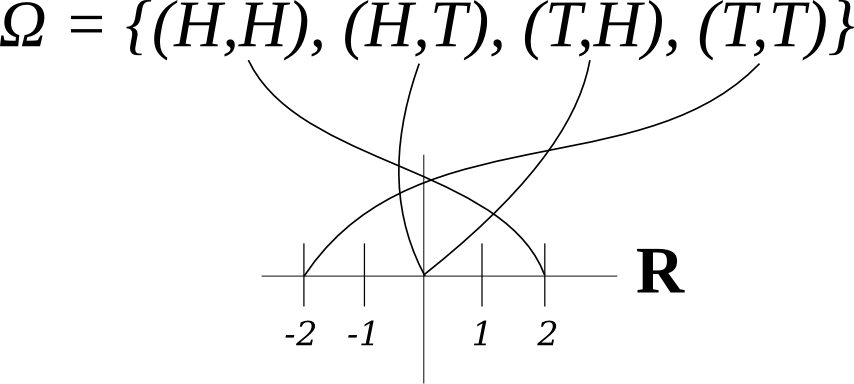
\includegraphics[width=.6\textwidth]{images/01set2nat}
	\caption{Members of a set being mapped to the natural numbers.}
	\label{fig:01set2nat}
\end{figure}

\section{Probability}
In this course $P$ means the probability measure on a set. $P: \Sigma \to [0,1]$ is a probability measure if given $A,B \in \Sigma$,
\begin{align*}
&A \cap B \in \emptyset \\
&P(A \cup B) = P(A) + P(B) \\
&A_i \in \Sigma ~ \forall ~ i \in \mathbb{N} \textnormal{ s.t. } A_i \cap A_j \neq \emptyset \textnormal{ if } i \neq j \\
&\Rightarrow P\left(\bigcup_{i=1}^\infty A_i\right) = \sum_{i=1}^\infty P(A_i).
\end{align*}
Given a R.V. $X$ then $F: \mathbb{R}^n \to [0,1]$ is the distribution function for $X$ if $F(x) = F\left((x_1,x_2,\ldots,x_n)\right) = \textnormal{``}P(X \leq x)\textnormal{''}$. More precisely we have $\textnormal{``}P(X \leq x)\textnormal{''} = P\left(\left\lbrace \omega \in \Omega | X(\omega) \leq x \right\rbrace \right)$. In this course inequalities are defined such that given $x, y \in \mathbb{R}^n$, if $x_i \leq y_i ~ \forall ~ i \in \lbrace 1,2,\ldots,n\rbrace$ then $x \leq y$. Using this definition we can restate the probability measure as
$$P\left(\left\lbrace \omega \in \Omega | X_1(\omega) \leq x_1, X_2(\omega) \leq x_2, \ldots, X_n(\omega) \leq x_n \right\rbrace \right).\footnote{This theorem is found in the text ``Probability'' by A. N. Shiryayev.}$$

If $F: \mathbb{R} \to [0,1]$ behaves such that $\lim_{x \to -\infty} F(x) = 0$, $\lim_{x \to +\infty} F(x) = 1$, $F$ is monotonically increasing and $F$ is right continuous (defined as $\lim_{y \downarrow x} F(y) = F(x)$) then $F$ is a distribution function for a R.V. Also, $f:\mathbb{R}^n \to [0,\infty]$ is a density function corresponding to the distribution $F$ if
$$F(x) = \int_{y \leq x} f(y)dy = \int_{-\infty}^{x_1} \int_{-\infty}^{x_2}\cdots \int_{-\infty}^{x_n} f(y_1,y_2,\ldots,y_n)dy_n\ldots dy_2dy_1.$$

\begin{example}
Given
\begin{align}
\label{eq:probEg}
\begin{split}
F(x) &= \begin{cases} 0 & x \leq 0 \\ 1-e^{-x} & x > 0 \end{cases} \\
f(x) &= \begin{cases} 0 & x \leq 0 \\ e^{-x} & x > 0 \end{cases}
\end{split}
\end{align}
Note that taking the indefinite integral of $f(x)$ yields $F(x)$.

There is a theorem that says if $X$ has a density $f$ then \\
``$P(A)$'' $= P\left(X^{-1}(A)\right) = \int_A f(x)dx$.
$\lozenge$
\end{example}

\section{Expectation}
The expectation of a R.V. taking a certain value is also known as the mean or average. Let $g: \mathbb{R}^n \to \mathbb{R}^m$, then
\begin{align*}
E[g(X)] &\doteq \int_{\mathbb{R}^n} g(x)f(x)dx \textnormal{ if } f ~ \exists \\
E[X] &= \int_{\mathbb{R}^n}xf(x)dx.
\end{align*}

\begin{example}
Using (\ref{eq:probEg}) we have
\begin{align*}
E[x] &= \int_{-\infty}^\infty xf(x)dx \\
&= \int_0^\infty xe^{-x}dx \\
&\quad [\text{use integration by parts with } u = x, dv = e^{-x}, v = -e^{-x}, du = 1] \\
&= -xe^{-x}\rvert_0^\infty + \int_0^\infty e^{-x}dx \\
&\quad [\text{use l'H\^opital's rule: } \lim_{x \to \infty} xe^{-x} = \lim_{x \to \infty} \frac{x}{e^x} = \lim_{x \to \infty} \frac{1}{e^x} = 0] \\
&= 0 - 0 - e^{-x}\rvert_0^\infty \\
&= 1.
\end{align*}
$\lozenge$
\end{example}

\section{Variance}
\begin{example}
Using (\ref{eq:probEg}) in $\mathbb{R}^1$ we have
$$E[(x - E(x))^2] = \int_0^\infty (x-1)^2e^xdx.$$
Since $x$ is a R.V. and $E(x)$ is a scalar the variance is a scalar as well.
$\lozenge$
\end{example}

\section{Covariance}
\begin{example}
Using (\ref{eq:probEg}) in $\mathbb{R}^n$ we have $$C_{ij} \doteq E[(x_i - E(x_i))(x_j - E(x_j)].$$ Note that $E(x_i) = \lbrace E(x) \rbrace_i$.
$\lozenge$
\end{example}

\begin{example}
Given
\begin{align*}
f(x) &= \begin{cases} 1 & x_1 \in [0,1] \\ 0 & x_2 \in [0,1] \end{cases} \\
E[x_1] &= \int_0^1 \int_0^1 x_1f(x_1,x_2)dx_1dx_2 = \int_0^1 \int_0^1 x_1dx_1dx_2 = \int_0^1 \frac{1}{2}dx_2 = \frac{1}{2}
\end{align*}
and by symmetry $E[x_2] = \frac{1}{2}$. This makes sense because we expect the value to be right in the middle of the area described by the function, as shown in Figure \ref{fig:01box}.
$\lozenge$
\end{example}

\begin{figure}[ht!]
	\centering
	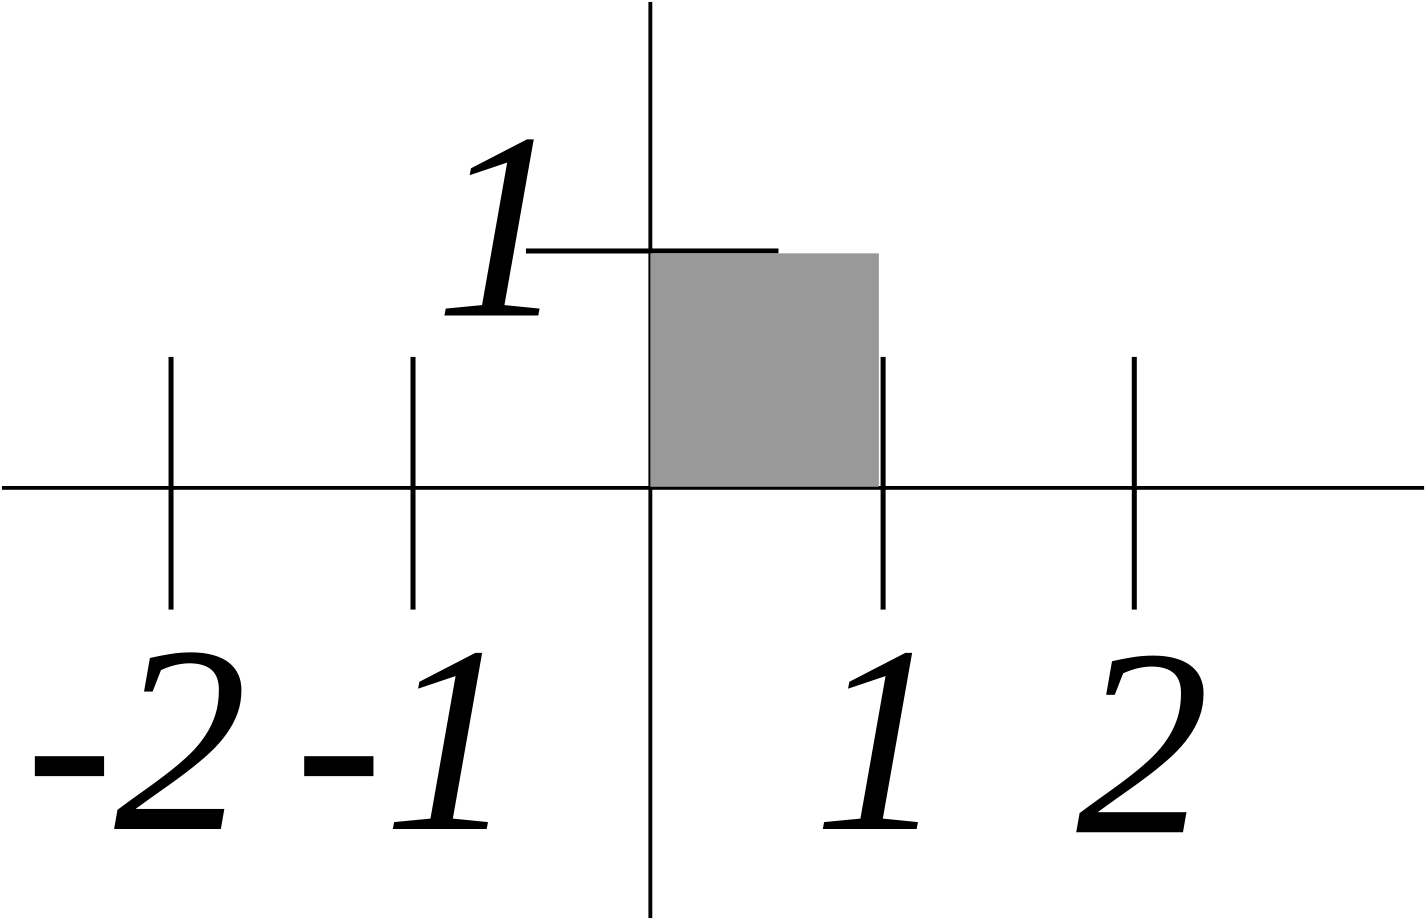
\includegraphics[width=.45\textwidth]{images/01box}
	\caption{The function $f(x)$.}
	\label{fig:01box}
\end{figure}

The off-diagonal elements of the covariance matrix can be calculated using
\begin{align*}
E[x] &= \frac{1}{2} \\
C_{12} &= E[(x_1 - \frac{1}{2})(x_2 - \frac{1}{2})] \\
&= \int_0^1 \int_0^1 (x_1 - \frac{1}{2})(x_2 - \frac{1}{2})dx_2dx_1 \\
&= \int_0^1 (x_1 - \frac{1}{2})[\int_0^1 (x_2 - \frac{1}{2})dx_2]dx_1 \\
&= \int_0^1 (x_1 - \frac{1}{2})[\underbrace{\int_0^1 x_2dx_2}_{= \frac{1}{2}} - \underbrace{\int_0^1 \frac{1}{2}dx_2}_{= \frac{1}{2}}]dx_1 \\
&= 0 \\
&\Rightarrow C = \left[\begin{array}{c c} s & 0 \\ 0 & s \end{array}\right]
\end{align*}
where $s$ is some scalar. Furthermore, we can see that \\
$C_{11} = \int_0^1\int_0^1(x_1-\frac{1}{2})^2dx_1dx_2$ leads to $s$ being a positive scalar because of the quadratic term inside the integrals.

\section{Gaussian Distribution}
A Gaussian distribution is also known as a normal distribution. To represent a R.V. $X$ as having a Gaussian distribution we write $X \sim \mathcal{N}(m,C)$, where $X \in \mathbb{R}^n$, $m \in \mathbb{R}^n$ and $C \in \mathbb{R}^{n \times m}$. $C_{n \times m}$ is a symmetric positive definite matrix if $X$ has a density of
\begin{align}
\label{eq:gaussDist}
f(x) = \frac{1}{(2\pi)^{n/2}|C|^{1/2}}e^{-\frac{1}{2}(x-m)^TC^{-1}(x-m)}
\end{align}
The Gaussian distribution is given by (\ref{eq:gaussDist}).

%%%%%%%%%%%%%%%%%%%%%%%%%%%%%%%%%%%%%%%%%%%%%%%%%%%%%%%%%%%%%
